% !TEX encoding = UTF-8 Unicode
\documentclass[12pt]{article}
\usepackage[usenames]{color}
\usepackage{amssymb} % maths
\usepackage{amsmath} % maths
\usepackage[utf8]{inputenc} % pour caracteres accentues
\usepackage[french]{babel}
\usepackage{graphicx}
\usepackage{url}
\usepackage{hyperref}


\usepackage{geometry} % pour la mise en page
\geometry{top=2cm, bottom=2cm, left=2cm, right=2cm}

\setlength{\parindent}{1cm} % alinea
\setlength{\parskip}{1ex plus 0.5ex minus 0.2ex} % espace entre paragraphs

\numberwithin{equation}{section} % numerotaion des equations

\newcommand{\HRule}{\rule{\linewidth}{0.5mm}} % barre horizontale


%%%%%%%%%%%%%%%%%%%%%%%%%%%%%%%%%%%%%%%%%%%%%%%%%%%%%%%%%%

\begin{document}


\thispagestyle{empty}

\phantom{.}
\vspace*{4cm}
\hspace*{-1.1cm} 
\HRule
 { \Huge \bfseries \center{Etude des catalogues COSMOS \\et True Universe \\à l'aide des Self Organizing Maps}\\[0cm] }
\rule{0cm}{0cm}
\\
\HRule 
\\ \\
\begin{center}
	\huge{Stage de Master Physique 1}
	\vspace{.5cm}
	\\ 2019 - 2020
	\vspace{1cm}
\end{center}



\begin{Large}
\noindent Encadrants : Alexandre BOUCAUD, 
\\ \hspace*{3cm} Hubert BRETONNIERE
\\
\\ Rapporteur : Yann RASERA
\\ \\
Stage effectué au sein du laboratoire Astroparticules \& Cosmologie sur une durée de 2 mois
\end{Large}



%%% Figure
\vspace{.5cm}
\begin{figure}[h!]
	\begin{minipage}[c]{.6\linewidth}
		\begin{Large}
		ROTH Olivier
		\end{Large}
	\end{minipage}
	\begin{minipage}[c]{.1\linewidth}
		\includegraphics[scale=0.1]{logo.png}
	\end{minipage}
\end{figure}



%%% Table of content
%%%%%%%%%%%%%%%%%%%%%%%%%%%%%%%%%%%%%%%%%%%%%%%%%%%%%%%%%%
\newpage
\thispagestyle{empty}
\tableofcontents



%%% Introduction
%%%%%%%%%%%%%%%%%%%%%%%%%%%%%%%%%%%%%%%%%%%%%%%%%%%%%%%%%%
\newpage
\thispagestyle{plain}
\setcounter{page}{1}

%\addcontentsline{toc}{section}{Introduction} 
\part*{Introduction}

Intro sur projet Euclid, "une mission destinée à percer les mystères de l’énergie noire et de la matière noire", d'après l'ESA

“Pour y parvenir, le satellite étudiera des galaxies qui se trouvent à différentes distances de la Terre au moyen d’un télescope de 1,2m de diamètre.\\ 
La mission tirera avantage du faible effet de lentille gravitationnelle, qui mesure la distorsion des galaxies lointaines causée par de la matière qui s’interpose, ainsi que des oscillations acoustiques des baryons, obtenues en mesurant l’agglomération des galaxies, pour obtenir une image en 3D de l’évolution de la distribution de la matière noire et de la matière ordinaire (baryonique) dans le cosmos."


veut identifier certains types de gx : on a donc besoin d'entrainer les algos à l'avance avec des données, pour savoir si ces données sont bien et pleinement représentatives de la réalité, on va comparer un catalogue issue d'une simulation avec un catalogue provenant de données réelles. afin de savoir si celui créé est bien représentatif de la réalité on veut visualiser des données et les SOMs sont un bon moyen

pk on a besoin / on introduit des SOMs ? : permet d'appréhender plus facilement des données à plusieurs dimension grâce à une map en 2D 


\vspace{2cm}
Intro sur les SOMs

Les Self Organizing Maps (SOMs, apprentissage non supervisé):
\\Ces réseaux utilisent essentiellement la quantification vectorielle pour détecter des patterns dans des données multidimensionnelles et les représenter dans des espaces à dimensions beaucoup plus faibles, généralement en deux dimensions.

La faible dimension de la carte résultante permet une présentation graphique des données qui peut être facilement interprétée par l'homme.





%%% Part 
%%%%%%%%%%%%%%%%%%%%%%%%%%%%%%%%%%%%%%%%%%%%%%%%%%%%%%%%%%
\newpage
\part{Théorie sur les SOMs}



Comme la plupart des réseaux neuronaux artificiels, les SOMs fonctionnent selon deux modes : l'entrainement et la cartographie."L'entrainement" construit la carte en utilisant des données d'entrée, tandis que la "cartographie" classifie automatiquement un nouveau vecteur d'entrée.

%%%
\textit{ reformuler paragraph précédent ; début ne colle pas avec le 2e paragraphe ; voire supprimer}
%%%
\vspace{1cm}


Les SOMs diffèrent des autres réseaux neuronaux artificiels car elles appliquent l'apprentissage compétitif par opposition à l'apprentissage par correction d'erreurs (comme la backpropagation avec descente de gradient), et dans le sens où elles utilisent une fonction de voisinage pour préserver les propriétés topologiques de l'espace d'entrée.


Les cartes obtenus sont constituées de neurones, disposés de façon rectangulaire ou hexagonale. Chaque neurone est associé à un vecteur “poids" ayant la même dimension que chaque vecteur d'entrée.


Alors que les neurones de l'espace cartographique restent fixes, l'entraînement consiste à déplacer des vecteurs de poids vers les données d'entrée (réduisant une métrique de distance) sans altérer la topologie induite de l'espace cartographique.  Ainsi, le SOM décrit une mise en correspondance d'un espace d'entrée de dimension supérieure à un espace cartographique de dimension inférieure. Une fois formée, la carte peut classer un vecteur de l'espace d'entrée en trouvant le neurone avec le vecteur de poids le plus proche du vecteur de l'espace d'entrée.


Les poids des neurones sont initialisés soit à de petites valeurs aléatoires, soit échantillonnés de manière égale depuis le jeu de données de l'entrée. Avec cette dernière alternative, l'apprentissage est beaucoup plus rapide car les poids initiaux donnent déjà une bonne approximation des poids du SOM.


 Pour s'assurer que ces modèles sont effectivement représentatifs des données sous-jacentes, il est essentiel d'évaluer la qualité des cartes.

\vspace{2cm}
%%%
\textit{peut-être des schémas à faire soi-même pour clarifier... 
\\ expliquer sigma et learning rate}
%%%


le sigma et le learning rate ralentissent tout deux au cours de l'entrainement pour affiner l'apprentissage. 



% SOM rect
\newpage
\section{Exemple avec un jeu de données de couleurs}
\begin{figure}[h!] 
	\center
	\label{fig1}
	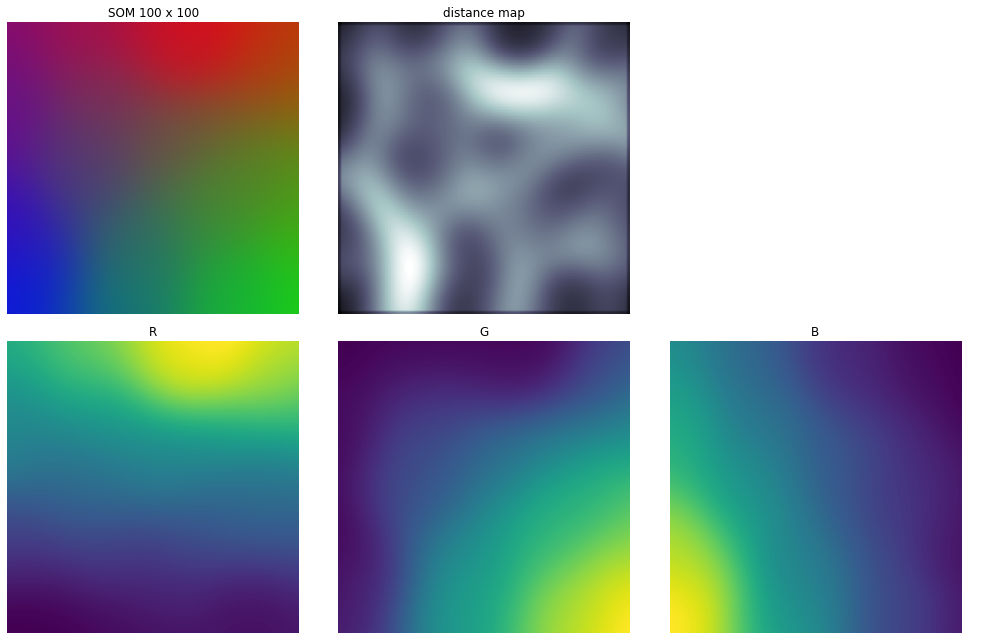
\includegraphics[width=\linewidth]{SOM_rect_norm_uniform.png}
	\caption{SOM topologie rectangulaire, distance map, poids de chaque couleur}
\end{figure}

On a pris un jeu de données uniforme de 250 000 couleurs, avec des perturbations (ici il y a un peu moins de rouge que de vert par exemple). Le sigma est à 10, un learning rate à 1 et on a entrainé sur 2000 itérations

À l'issue de l'entrainement les couleurs sont classées comme on peut le voir sur le graphique en haut à gauche de la figure \ref{fig1}.

Les poids de chaque couleur, les trois graphiques en bas, sont bien dissociés et chaque couleur est formée d'un seul cluster.

La distance map nous permet de voir les limites entre les couleurs. Si deux couleurs proches dans le spectre se trouve à côté alors leur distance sera faible et le pixel représentant cette distance sur la distance map sera foncé.



% SOM hexa
\newpage
On peut également faire un entrainement avec une topologie hexagonale. le résultat est censé être meilleur puisque chaque neurone possède 6 voisin direct au lieu de 4 dans une topologie rectangulaire, facilitant les déplacement / agencements.
\begin{figure}[h!] 
	\center
	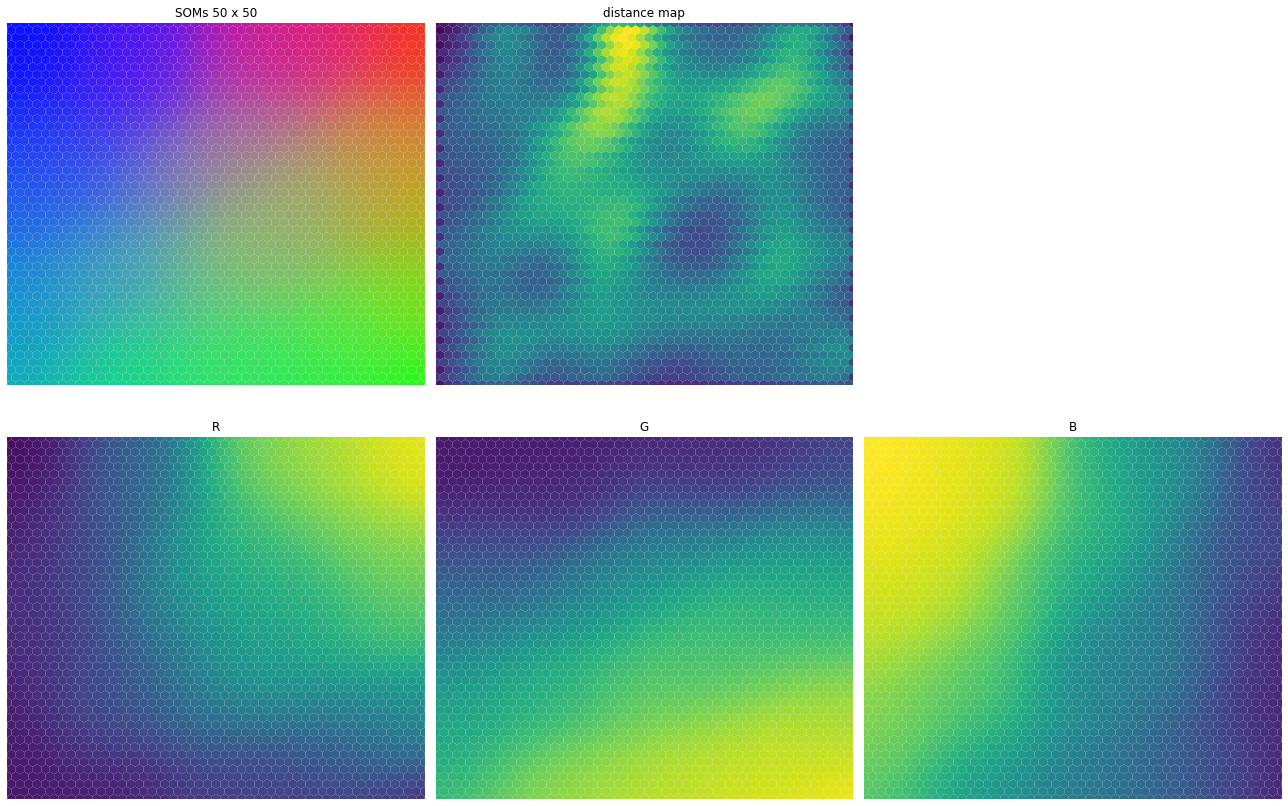
\includegraphics[width=12cm]{SOM_hexa_norm_uniform.png}
	\caption{SOM topologie hexagonale, distance map, poids de chaque couleur}
\end{figure}

Avec notre jeu de données normalisé, on observe une belle répartition des couleurs et une distance map assez faible dans l'ensemble. Chaque couleur est constitué d'un seul cluster et est bien distincte des autres.




\newpage
\section{parler des erreurs ? convergence ?}


quantization error, topological error, neighborhood preservation, trustworthiness



\section{utilité de l'entrainement avec des couleurs : la heatmap (visualisation de l'activation des neurones etc)}


\noindent On regarde où tombe un jeu de données de 10 000 couleurs majoritairement bleues à 0.7 sur la SOM précédente :



%%% Figure
\vspace{.5cm}
\begin{figure}[h!]
	\begin{minipage}[l]{.5\linewidth}
		\includegraphics[scale=0.77]{SOM_rect_norm_uniform_B}
		\caption{weight blue}
	\end{minipage}
	\begin{minipage}[r]{.5\linewidth}
		\includegraphics[scale=0.25]{heatmap.png}
		\caption{Heatmap }
	\end{minipage}
\end{figure}


On voit que notre jeu de données majoritairement bleu tombe bien la où le bleu est réparti sur la map.
Puisqu'on a pris du bleu soft, gaussien en 0.7 un peu de rouge et de vert, les points de la heatmap ne sont pas à l'extrémité du bleu du SOM.

Chaque neurone a été activé un certain nombre de fois, ce nombre est présent sur les pixels de la heatmap.




%%% Part 
%%%%%%%%%%%%%%%%%%%%%%%%%%%%%%%%%%%%%%%%%%%%%%%%%%%%%%%%%%
\newpage
\part{Application des SOMs aux catalogues COSMOS et True Universe}


\noindent Evolution croisée de l'indice de sersic et de l'ellipticité pour le catalogue COSMOS

\begin{figure*}[h!]
	\center
	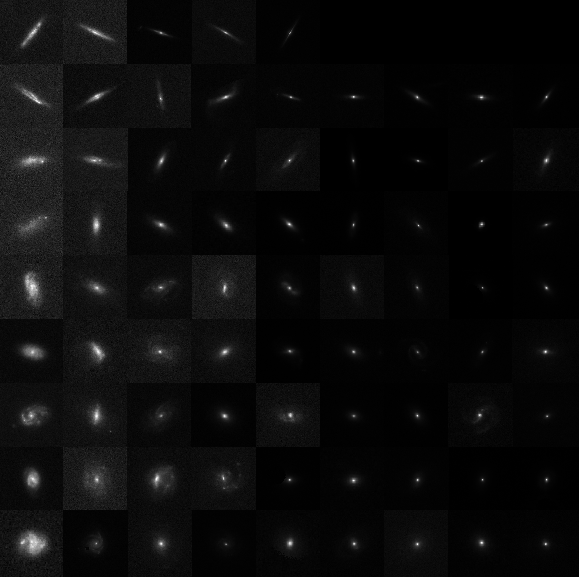
\includegraphics{GxCOSMOS}
\end{figure*}



















%%% Références
%%%%%%%%%%%%%%%%%%%%%%%%%%%%%%%%%%%%%%%%%%%%%%%%%%%%%%%%%%
\newpage
\thispagestyle{empty}



\begin{thebibliography}{1}	% use \cite{cite key .} in the document to make a link
	\bibitem{ESA} European Space Agency, Mission Euclid : \url{https://www.esa.int/Space_in_Member_States/France/Euclid_une_mission_destinee_a_percer_les_mysteres_de_l_energie_noire_et_de_la_matiere_noire}.
	\bibitem{cite key 1} Author. \textit{Title}.  year
	\bibitem{cite key 2} Bibliothèque Minisom sur Github \url{ https://github.com/JustGlowing/minisom}
	\bibitem{cite key 3} Gregory T. Breard, Thèse : \textit{Evaluating Self-Organizing Map Quality Measures as Convergence Criteria}, 2017, Université de Rhode Island.

\end{thebibliography}





%%% Annexe
%%%%%%%%%%%%%%%%%%%%%%%%%%%%%%%%%%%%%%%%%%%%%%%%%%%%%%%%%%
\newpage
\part*{Annexe}


growing SOMs : à mettre si visualisation réussie

recherche d'optimisation des paramètres avec hyperparams


obtenir plus d'infos sur les SOMs : regarder et quantifier les différentes erreurs, optimisation, regroupement à la fin de l'entrainement (avec SOMperf)





\end{document}